\documentclass[11pt,class=report,crop=false]{standalone}
\usepackage[screen]{../python}


\begin{document}


%====================================================================
\chapitre{Nombres complexes II}
%====================================================================

\objectifs{On poursuit l'exploration des nombres complexes en se concentrant sur la forme module/argument.}

\index{nombre complexe}

%%%%%%%%%%%%%%%%%%%%%%%%%%%%%%%%%%%%%%%%%%%%%%%%%%%%%%%%%%%%%%%%
%%%%%%%%%%%%%%%%%%%%%%%%%%%%%%%%%%%%%%%%%%%%%%%%%%%%%%%%%%%%%%%%

\begin{cours}[Nombres complexes]

\index{nombre complexe!module}
\index{nombre complexe!argument}

\textbf{Module/argument.}
Tout nombre complexe $z \in \Cc^{\ast}$, s'écrit :
$$z = r \left( \cos \theta +  i \sin \theta \right)$$
où 
\begin{itemize}
  \item $r = \left| z \right|$ est le module de $z$,
  \item et $\theta \in \Rr$ est un \defi{argument}.%\index{argument}
\end{itemize}


\myfigure{1}{
\tikzinput{fig-complexes2-1}
}


\medskip
\textbf{Unicité.}
Si $\theta$ est un argument, alors n'importe quel $\theta + 2k\pi$ est aussi un argument.

Pour éviter cette indécision, on peut imposer à $\theta$ d'appartenir à l'intervalle $]-\pi,+\pi]$, l'argument est alors unique. 
Pour $z \in \Cc^*$, il existe un unique couple $(r,\theta)$ avec $r>0$ et $\theta \in ]-\pi,+\pi]$ tel que :
$$z = r \left( \cos \theta +  i \sin \theta \right).$$


\emph{Remarques.}
\begin{itemize} 
  \item Une autre convention aurait été de choisir l'intervalle $[0,2\pi[$. 
  \item L'écriture $(r,\theta)$ s'appelle aussi l'écriture en coordonnées polaires d'un nombre complexe, par opposition à l'écriture $z=a+ib$ qui est l'écriture cartésienne.
\end{itemize}

\end{cours}


%%%%%%%%%%%%%%%%%%%%%%%%%%%%%%%%%%%%%%%%%%%%%%%%%%%%%%%%%%%%%%%%
%%%%%%%%%%%%%%%%%%%%%%%%%%%%%%%%%%%%%%%%%%%%%%%%%%%%%%%%%%%%%%%%

\begin{cours}[Module \texttt{cmath}]

\index{nombre complexe!cmath@\ci{cmath}}
\index{module!cmath@\ci{cmath}}

Le module \ci{cmath} fournit des outils supplémentaires pour les nombres complexes.
Pour éviter les conflits avec le module \ci{math} nous l'importerons par :
\mycenterline{\ci{import cmath}}


\begin{enumerate}

  \item \ci{cmath.phase(z)}\index{phase@\ci{phase}} renvoie l'argument $\theta \in ]-\pi,+\pi]$ du nombre complexe $z$.
  Exemple : \ci{cmath.phase(1-1j)} renvoie  \ci{-0.785...} qui correspond à la valeur $-\frac\pi4$.  
  
  \item Rappel : \ci{abs(z)} renvoie le module $|z|$ (c'est une fonction interne à \Python).
   
  \item \ci{cmath.polar(z)}\index{polar@\ci{polar}} renvoie le couple module/argument $(r,\theta)$.
  Exemple : \ci{cmath.polar(1-1j)} renvoie \ci{(1.414..., -0.785...)} qui correspond au couple 
  $(r,\theta) = (\sqrt2,-\frac\pi4)$.
  
  \item \ci{cmath.rect(r,theta)}\index{rect@\ci{rect}} renvoie le nombre complexe dont le module est $r$ et l'argument $\theta$. Exemple : \ci{cmath.rect(2,pi/4)} renvoie \ci{1.414... + 1.414...j} et correspond à $\sqrt{2}+i\sqrt{2}$.

\end{enumerate}  
\end{cours}

%%%%%%%%%%%%%%%%%%%%%%%%%%%%%%%%%%%%%%%%%%%%%%%%%%%%%%%%%%%%%%%%
% Activité 1
%%%%%%%%%%%%%%%%%%%%%%%%%%%%%%%%%%%%%%%%%%%%%%%%%%%%%%%%%%%%%%%%

\begin{activite}[Module/argument]

\objectifs{Objectifs : utiliser \Python{} pour calculer et mieux comprendre la forme module/argument.}

\begin{enumerate}
  \item Pour un nombre complexe $z$, par exemple $z=1+3i$ ou $z=1+i$, calcule son module et son argument à l'aide de \Python. 
  
  \item Quel nombre complexe a pour module $2$ et argument $\frac\pi3$ ? Même question pour le complexe de module $3$ et d'argument $\frac{3\pi}{2}$. Essaie de deviner la réponse exacte à partir des valeurs approchées données par \Python.
  
  \item \`A l'aide du module \ci{matplotlib}, place le point d'affixe $z$ dont on te donne le module et l'argument, par exemple de module $\sqrt2$ et argument $\frac\pi6$.
  
  \item Soit $n\ge3$. Soit $\omega$ le nombre complexe de module $1$ et d'argument $\frac{2\pi}{n}$. 
  Trace le polygone ayant pour sommets les points d'affixes :
  $$1, \omega, \omega^2, \ldots, \omega^{n-1}.$$
  Quelle est la nature de ce polygone ?
  
  
\begin{center}
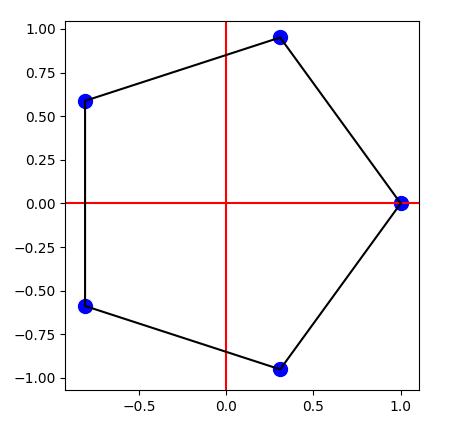
\includegraphics[scale=\myscale,scale=0.5]{ecran-complexes2-1}
\end{center}	 
  
   
\end{enumerate} 
\end{activite}


%%%%%%%%%%%%%%%%%%%%%%%%%%%%%%%%%%%%%%%%%%%%%%%%%%%%%%%%%%%%%%%%
% Activité 2
%%%%%%%%%%%%%%%%%%%%%%%%%%%%%%%%%%%%%%%%%%%%%%%%%%%%%%%%%%%%%%%%

\begin{activite}[Module/argument (suite)]

\objectifs{Objectifs : créer tes propres fonctions qui permettent la conversion entre l'écriture cartésienne d'un nombre complexe et son écriture sous la forme module/argument.}

Tu vas écrire tes propres fonctions pour calculer avec les modules et les arguments.

\begin{enumerate}
  \item Programme une fonction \ci{polaire_vers_cartesien(module,argument)} qui renvoie le nombre complexe $z$ (sous la forme d'un nombre complexe \Python) dont le module et l'argument sont donnés.
  Utilise la formule 
  $$z = r\cos\theta + ir\sin\theta.$$
  Compare ton résultat avec la fonction \ci{rect} du module \ci{cmath}.
  
  
  \item Programme une fonction \ci{cartesien_vers_polaire(z)} qui renvoie le module et l'argument du nombre complexe $z$.
Récupère d'abord la partie réelle $x$ et la partie imaginaire $y$ de $z$. 
Le module est alors facile à calculer. L'argument se calcule par la formule :
$$\theta = \operatorname{atan2}(y,x)$$
La fonction \ci{atan2} est une variante de la fonction \og{}arctangente\fg{} et est disponible dans le module \ci{math}.

  Compare ta fonction avec les fonctions \ci{phase} et \ci{polar} du module \ci{cmath}.
  
  \item Programme une fonction \ci{argument_dans_intervalle(angle)} qui renvoie une mesure de l'angle dans l'intervalle $]-\pi,+\pi]$. Par exemple soit $\theta = \frac{5\pi}{2}$,  
 comme $\theta = -\frac\pi2 + 3 \cdot 2\pi$ alors $\theta'= -\frac\pi2$ est la mesure de l'angle dans l'intervalle $]-\pi,+\pi]$.
 
 \emph{Indication.} Commence par ramener l'angle dans l'intervalle $[0,2\pi[$, puis discute selon la valeur.
 
 Une fois terminé compare ton résultat avec la commande \ci{angle \% 2*pi}.

\end{enumerate} 
\end{activite}

\begin{cours}[Notation exponentielle]
	\index{exponentielle complexe}
\sauteligne
\begin{itemize}
  \item \textbf{Notation exponentielle.}
  On note 
  $$e^{i\theta} = \cos(\theta) + i \sin(\theta).$$
  C'est donc le nombre complexe de module $1$ et d'argument $\theta$. 
  
  
  \item \textbf{Formules d'Euler.} Un petit calcul conduit à :
$$ \cos \theta = \frac{e^{i  \theta} + e^{- i  \theta}}{2} \quad \text{ et } \quad
   \sin \theta = \frac{e^{i  \theta} - e^{- i  \theta}}{2 i }.$$

  \item \textbf{Formule de Moivre.}
  
  $$\left( \cos \theta + i \sin \theta \right)^n = \cos \left( n \theta \right)
  + i  \sin \left( n \theta \right).$$
  
  Avec la notation exponentielle, l'écriture de cette formule est très simple :
  $$\left(e^{i\theta}\right)^n = e^{i n \theta}.$$
  
\end{itemize}
\end{cours}

%%%%%%%%%%%%%%%%%%%%%%%%%%%%%%%%%%%%%%%%%%%%%%%%%%%%%%%%%%%%%%%%
% Activité 3
%%%%%%%%%%%%%%%%%%%%%%%%%%%%%%%%%%%%%%%%%%%%%%%%%%%%%%%%%%%%%%%%

\begin{activite}[Euler, de Moivre, Gauss]

\objectifs{Objectifs : mettre en \oe uvre plusieurs formules.}

\begin{enumerate}
  \item \textbf{Euler.} Programme deux fonctions \ci{cosinus(t)} et \ci{sinus(t)} qui calculent et renvoient le cosinus et le sinus d'un réel $t$ donné en utilisant les formules d'Euler.
  
 \emph{Indication.} Utilise ta fonction \ci{polaire_vers_cartesien()} de l'activité 1 pour calculer $e^{it}$. 
  
  \emph{Exemple.} Retrouve le sinus et le cosinus de $t = \frac\pi6$.
  
%  \emph{Remarque.} Ce n'est pas vraiment une nouvelle façon de calculer des sinus et des cosinus car pour le passage des vers les coordonnées cartésienne on utilise ces fonctions.
     
  
  \item \textbf{de Moivre.} Programme une fonction \ci{puissance_bis(z,n)} qui calcule $z^n$ à l'aide de la formule de Moivre selon le principe suivant :
  \begin{itemize}
    \item \'Ecrire $z$ sous la forme $z = r e^{i\theta}$ (utilise ta fonction \ci{cartesien_vers_polaire()}).
    \item Calculer $r^n$ et $n\theta$.
    \item Renvoyer $z^n$ grâce à la formule de Moivre $z^n = r^n e^{in\theta}$
     (utilise ta fonction \ci{polaire_vers_cartesien()}).
  \end{itemize}
  \emph{Exemple.} Calcule $(2-3i)^{10}$. 
  
  \emph{Complexité.} La formule de Moivre permet de remplacer le calcul d'une puissance d'un nombre complexe par le calcul de la puissance d'un nombre réel (son module).
  
  \item \textbf{Gauss.} Comment calculer plus rapidement le produit de deux nombres complexes ?
  Soit $z=a+ib$ et $z'=c+id$. La formule naïve donnée par la définition est :
  $$z \times z' = (ac-bd) + i(ad+bc).$$
  Pour calculer un produit de deux nombres complexes, il faut donc calculer le produit de $4$ nombres réels : $ac$, $bd$, $ad$, $bc$.
  
  Nous allons voir deux méthodes, dues à Gauss, qui ne nécessitent que $3$ multiplications de nombres réels.
  
  \textbf{Méthode 1.}
  Calculer $r=ac$, $s = bd$, $t = (a+b)(c+d)$, alors $z = (r-s) + i(t-r-s)$.
  
  \textbf{Méthode 2.}
  Calculer $r = c(a+b)$, $s = a(d-c)$, $t = b(c+d)$, alors  $z = (r-t) + i(r+s)$.

  Programme trois fonctions du type \ci{multiplication(a,b,c,d)} qui renvoient la partie réelle et la partie imaginaire de $(a+ib)\times(c+id)$ par les trois méthodes décrites ici.
 Teste tes fonctions en calculant $(2+5i)\times(3-2i)$.  
  
\end{enumerate} 
\end{activite}


%%%%%%%%%%%%%%%%%%%%%%%%%%%%%%%%%%%%%%%%%%%%%%%%%%%%%%%%%%%%%%%%
% Activité 4
%%%%%%%%%%%%%%%%%%%%%%%%%%%%%%%%%%%%%%%%%%%%%%%%%%%%%%%%%%%%%%%%

\begin{activite}[Cercles et droites]

\objectifs{Objectifs : tracer des cercles et des droites en utilisant les nombres complexes.}

\begin{enumerate}
  \item Programme une fonction \ci{affiche_liste(zliste)} qui trace et affiche les points 
  d'affixe $z$ donnés dans la liste.
  
  \emph{Indication.} Utilise la commande \ci{plt.scatter(x,y)} provenant de \ci{matplotlib}.
  C'est encore mieux si tu autorises les arguments optionnels avec une entête du type 
  \ci{affiche_liste(zliste,couleur='blue',taille=10)}.
  
  
  \item Programme une fonction \ci{trace_cercle(z0,r)} qui renvoie une liste de complexes $z$ appartenant au cercle centré en $z_0$ et de rayon $r$.
  
  \emph{Indications.}
  \begin{itemize} 
    \item Ces complexes $z$ vérifient $|z-z_0|=r$ et sont donc de la forme :
    $$z = r e^{2i\pi\theta}, \qquad 0 \le \theta < 1.$$
    \item C'est mieux d'avoir en argument optionnel le nombre de points avec une entête du type \ci{trace_cercle(z0,r,numpoints=100)}.
    
    \item Trace le cercle à l'aide de ta fonction \ci{affiche_liste()}.
   \end{itemize} 
   
  
\begin{center}
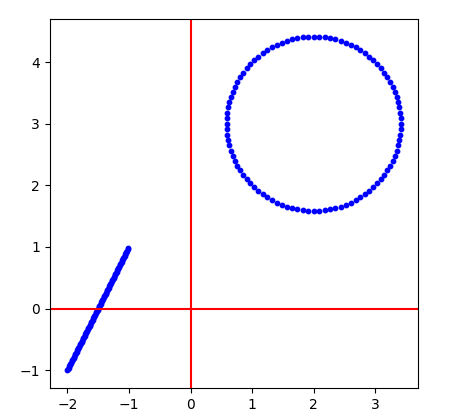
\includegraphics[scale=\myscale,scale=0.5]{ecran-complexes2-4}
\end{center}
\emph{Figure.} Voici le cercle de centre $2+3i$ et de rayon $\sqrt2$, ainsi que le segment entre les points d'affixes $-2-i$ et $-1+3i$.
 
   
   \item Programme une fonction \ci{trace_segment(z0,z1)}
  qui renvoie une liste de complexes $z$ appartenant au segment $[z_0,z_1]$.
  
  \emph{Indications.}
  \begin{itemize} 
    \item Ces complexes $z$ vérifient $z \in[z_0,z_1]$ et sont donc de la forme :
    $$z = (1-t)z_0 + tz_1, \qquad 0 \le t \le 1.$$
    \item C'est mieux d'avoir le nombre de points en argument optionnel avec une entête du type \ci{trace_segment(z0,z1,numpoints=100)}.
    
    \item Trace le segment à l'aide de ta fonction \ci{affiche_liste()}.
   \end{itemize}   
   
\end{enumerate} 
\end{activite}


%%%%%%%%%%%%%%%%%%%%%%%%%%%%%%%%%%%%%%%%%%%%%%%%%%%%%%%%%%%%%%%%
% Activité 5
%%%%%%%%%%%%%%%%%%%%%%%%%%%%%%%%%%%%%%%%%%%%%%%%%%%%%%%%%%%%%%%%

\begin{activite}[Transformations du plan]

\objectifs{Objectifs : définir des transformations du plan à l'aide des nombres complexes.}

\begin{enumerate}
  \item Programme les fonctions suivantes. Chaque fonction est du type
  \ci{transformation(zliste)} et renvoie la liste des $f(z)$ pour $z$ parcourant la liste donnée :
  \begin{itemize}
    \item une fonction \ci{translation(zliste,v)} qui correspond à la translation $z \mapsto z + v$, où $v\in\Cc$ est fixé,
    
    \item une fonction \ci{homothetie(zliste,k)} qui correspond à l'homothétie de centre $0$ et de rapport $k\in\Rr$ : $z \mapsto kz$,
    
    \item une fonction \ci{rotation(zliste,theta)} qui correspond à la rotation d'angle $\theta$, centrée en $0$ : $z \mapsto ze^{i\theta}$,
    
    \item une fonction \ci{symetrie(zliste)} qui correspond à la symétrie axiale $z \mapsto \bar z$.
    
  \end{itemize}
  
Affiche ensuite l'image d'un cercle et d'un carré pour chacune de ces transformations (un carré est formé de quatre segments !). Ci-dessous un cercle et un carré \couleurnb{(en bleu) }{}et leur image pour chaque transformation\couleurnb{ (en rouge)}{}.
   
\begin{center}
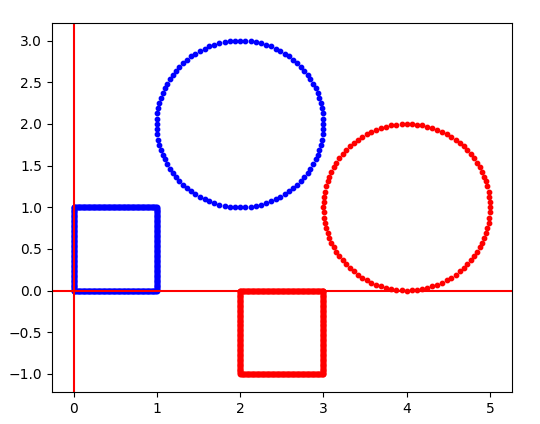
\includegraphics[scale=\myscale,scale=0.4]{ecran-complexes2-5a}\quad
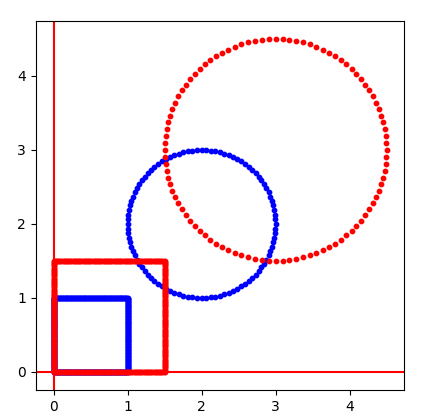
\includegraphics[scale=\myscale,scale=0.4]{ecran-complexes2-5b}

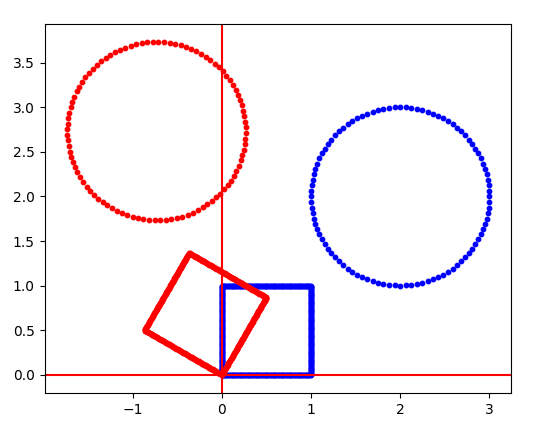
\includegraphics[scale=\myscale,scale=0.4]{ecran-complexes2-5d}\quad
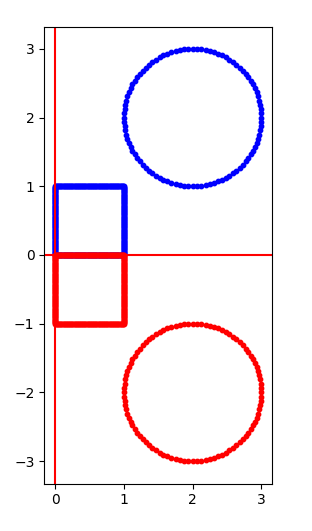
\includegraphics[scale=\myscale,scale=0.4]{ecran-complexes2-5c}

\end{center}  
  
  
  \item  Programme une fonction \ci{inversion(zliste)} qui correspond à l'inversion qui est l'application $z \mapsto \frac1 z$ (pour $z \in \Cc^*$).
  
  En particulier essaie de conjecturer en quoi est transformée une droite, en quoi est transformé un cercle (les cas où la droite ou le cercle passent par l'origine sont spéciaux).
  
   Ci-dessous un cercle et un carré\couleurnb{ (en bleu)}{} et leur image par l'inversion\couleurnb{ (en rouge)}{}.
\begin{center}
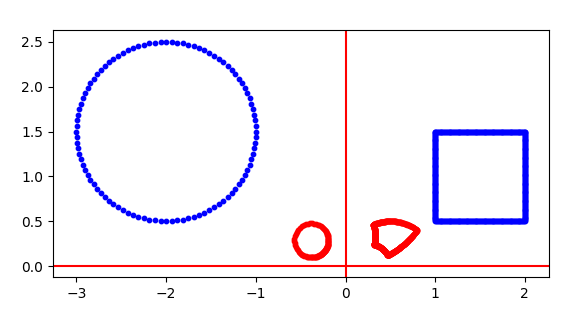
\includegraphics[scale=\myscale,scale=0.5]{ecran-complexes2-5e}
\end{center}   

  \item  Programme une fonction \ci{au_carre(zliste)} qui correspond à l'application $z \mapsto z^2$.
 
   Ci-dessous un cercle et un carré\couleurnb{ (en bleu)}{} et leur image\couleurnb{ (en rouge)}{}.
\begin{center}
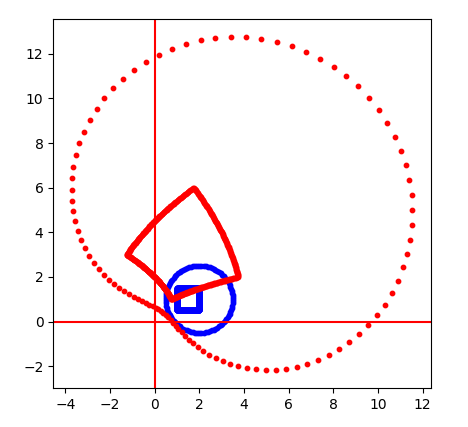
\includegraphics[scale=\myscale,scale=0.5]{ecran-complexes2-5f}
\end{center}  
  
\end{enumerate} 
\end{activite}


\end{document}
